

\title{Project title}
\author{Yangkang Chen}

\renewcommand{\thefootnote}{\fnsymbol{footnote}}

\author{Yangkang Chen\footnotemark[1]}

\ms{GEO-2018} %\ms{GJI-2018}

\address{
\footnotemark[1]
School of Earth Sciences\\
Zhejiang University\\
Hangzhou, Zhejiang Province, China, 310027\\
yangkang.chen@zju.edu.cn 
}

\lefthead{Chen et al., 2018}
\righthead{PROJNAME}

\begin{abstract}
A brief summary of the work.
\end{abstract}

%\section{Keywords}
%key1,key2,key3

\section{Introduction}
\section{Theory}
\section{Examples}
\section{Discussions}
\section{Conclusions}
\section{Acknowledgements}

%\inputdir{test}
%\plot{test1}{width=\textwidth}{Separated x-component of the S1 elastic wavefield in the orthorhombic media.}
%\multiplot{2}{test1,test2}{width=0.45\textwidth}{(a) Caption a. (b) Caption b.}




\bibliographystyle{seg}
\bibliography{projname}

%\AtEndDocument{}

%\newpage
%\listoffigures



%\begin{figure}[htb!]
%	\centering
%	\subfloat[]{\includegraphics[width=0.8\textwidth]{Fig/fig}}
%	\caption{Caption.}
%	\label{fig:fig}
%\end{figure}

%\begin{figure}[htb!]
%	\centering
%	\subfloat[]{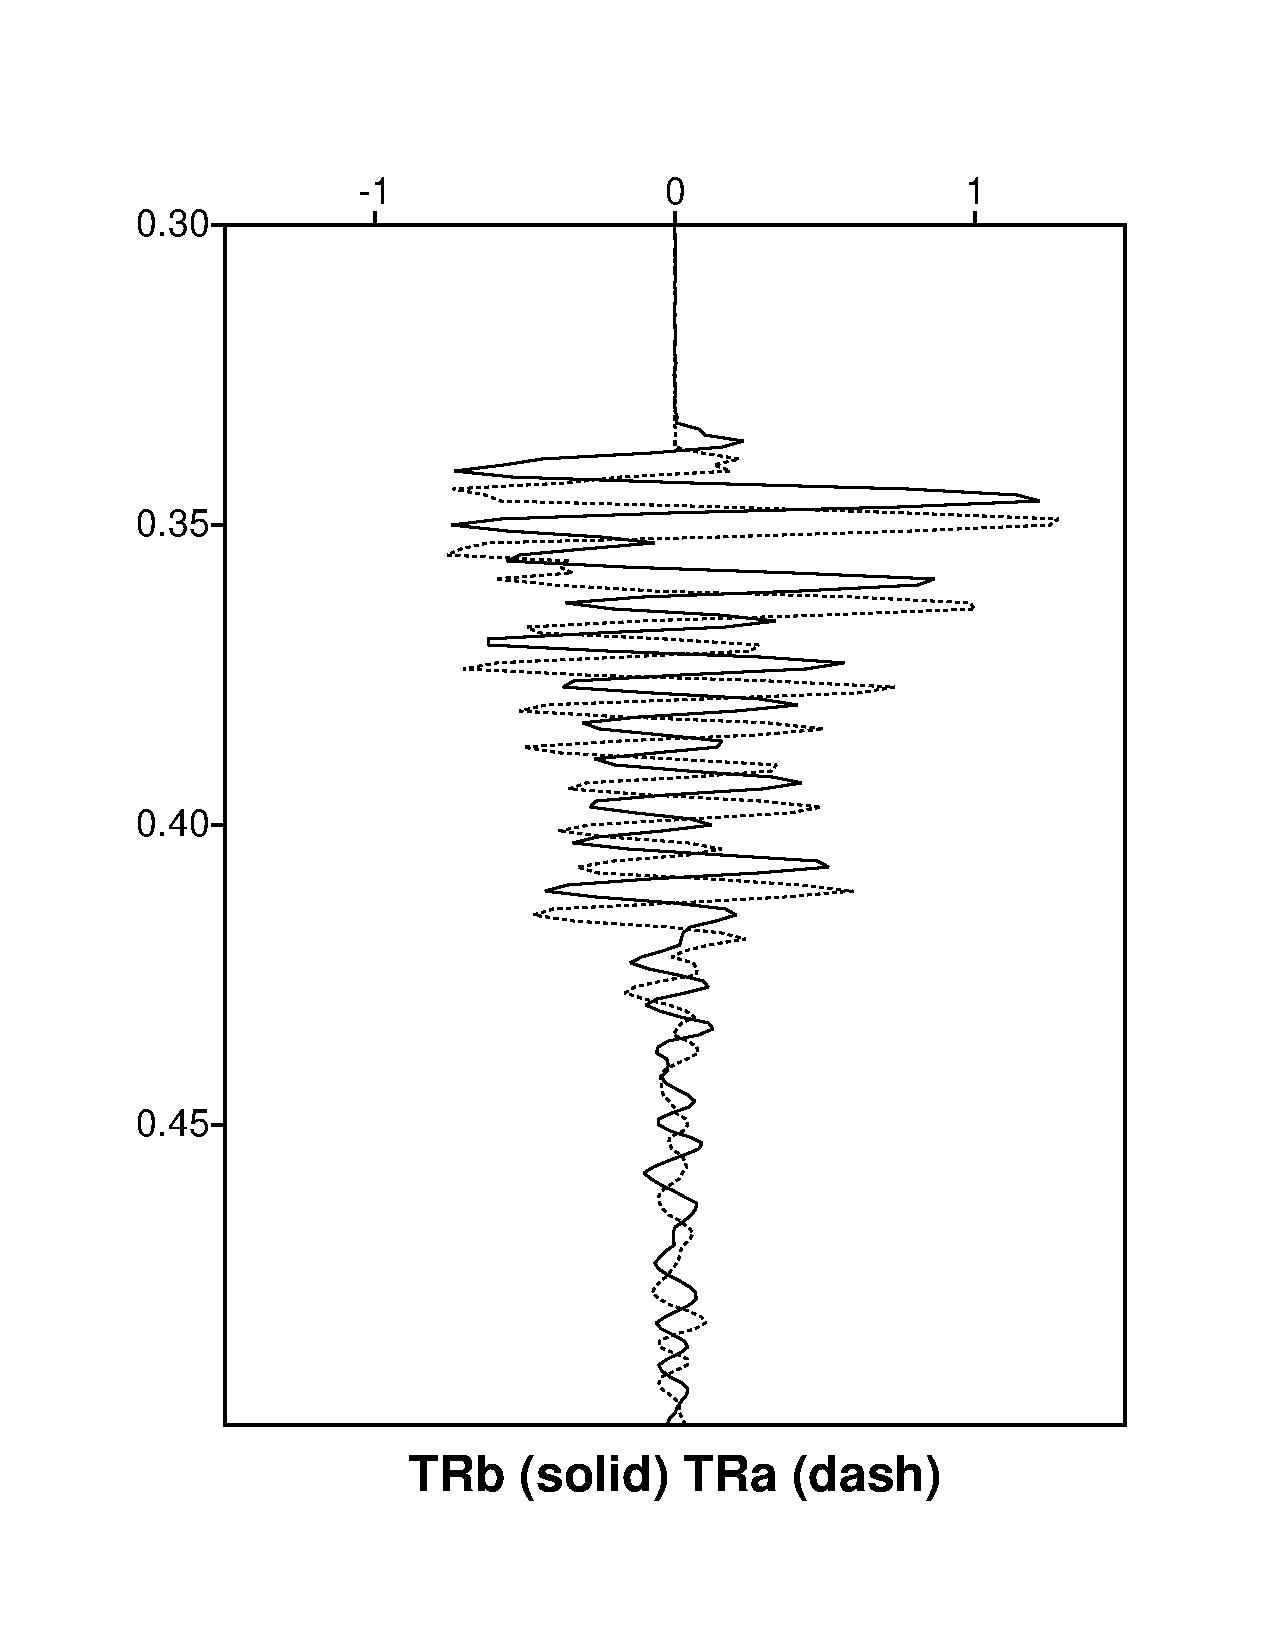
\includegraphics[width=0.45\textwidth]{Fig/fig1}
%    \label{fig:fig1}}\\
%    \subfloat[]{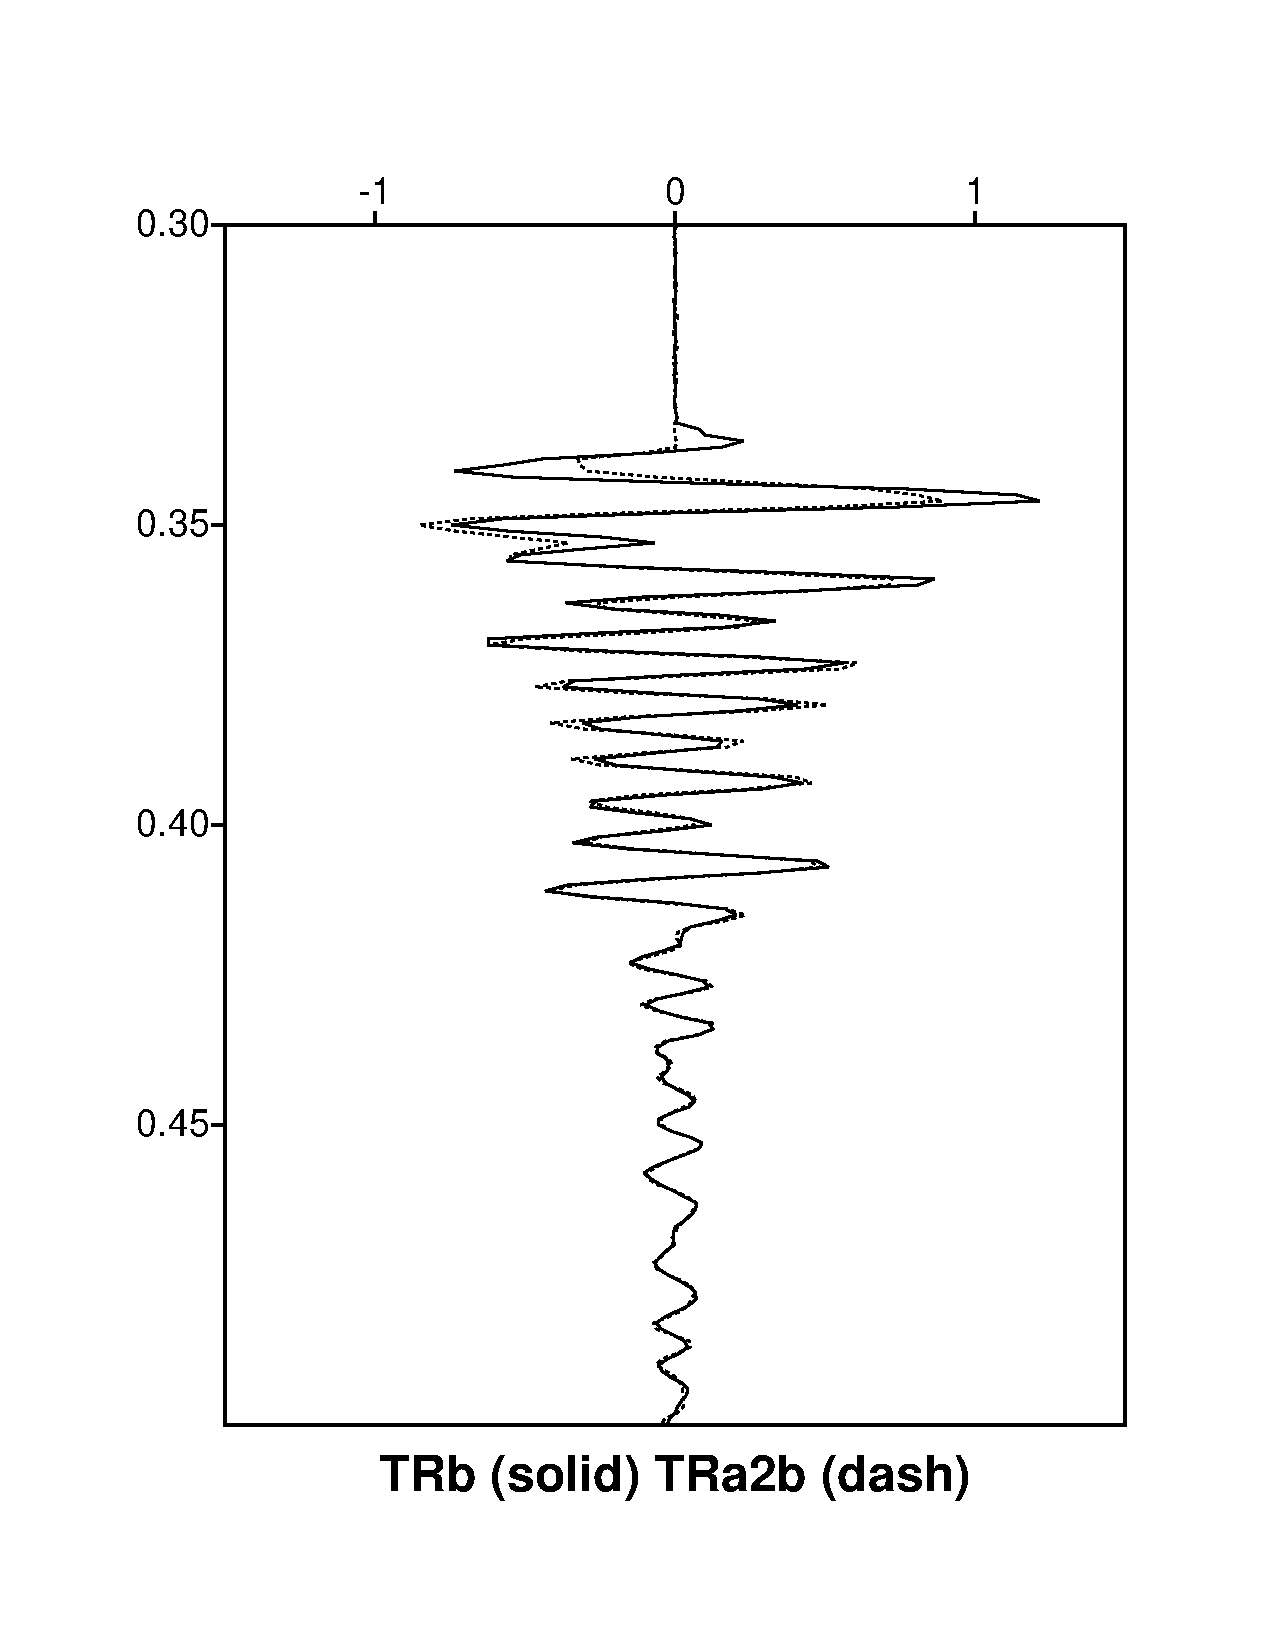
\includegraphics[width=0.45\textwidth]{Fig/fig2}
%    \label{fig:fig2}}\\
%	\caption{(a) Caption a. (b) Caption b.}
%	\label{fig:fig1,fig2}
%\end{figure}

%\begin{figure*}[ht!]
%	\centering
%	\subfloat[]{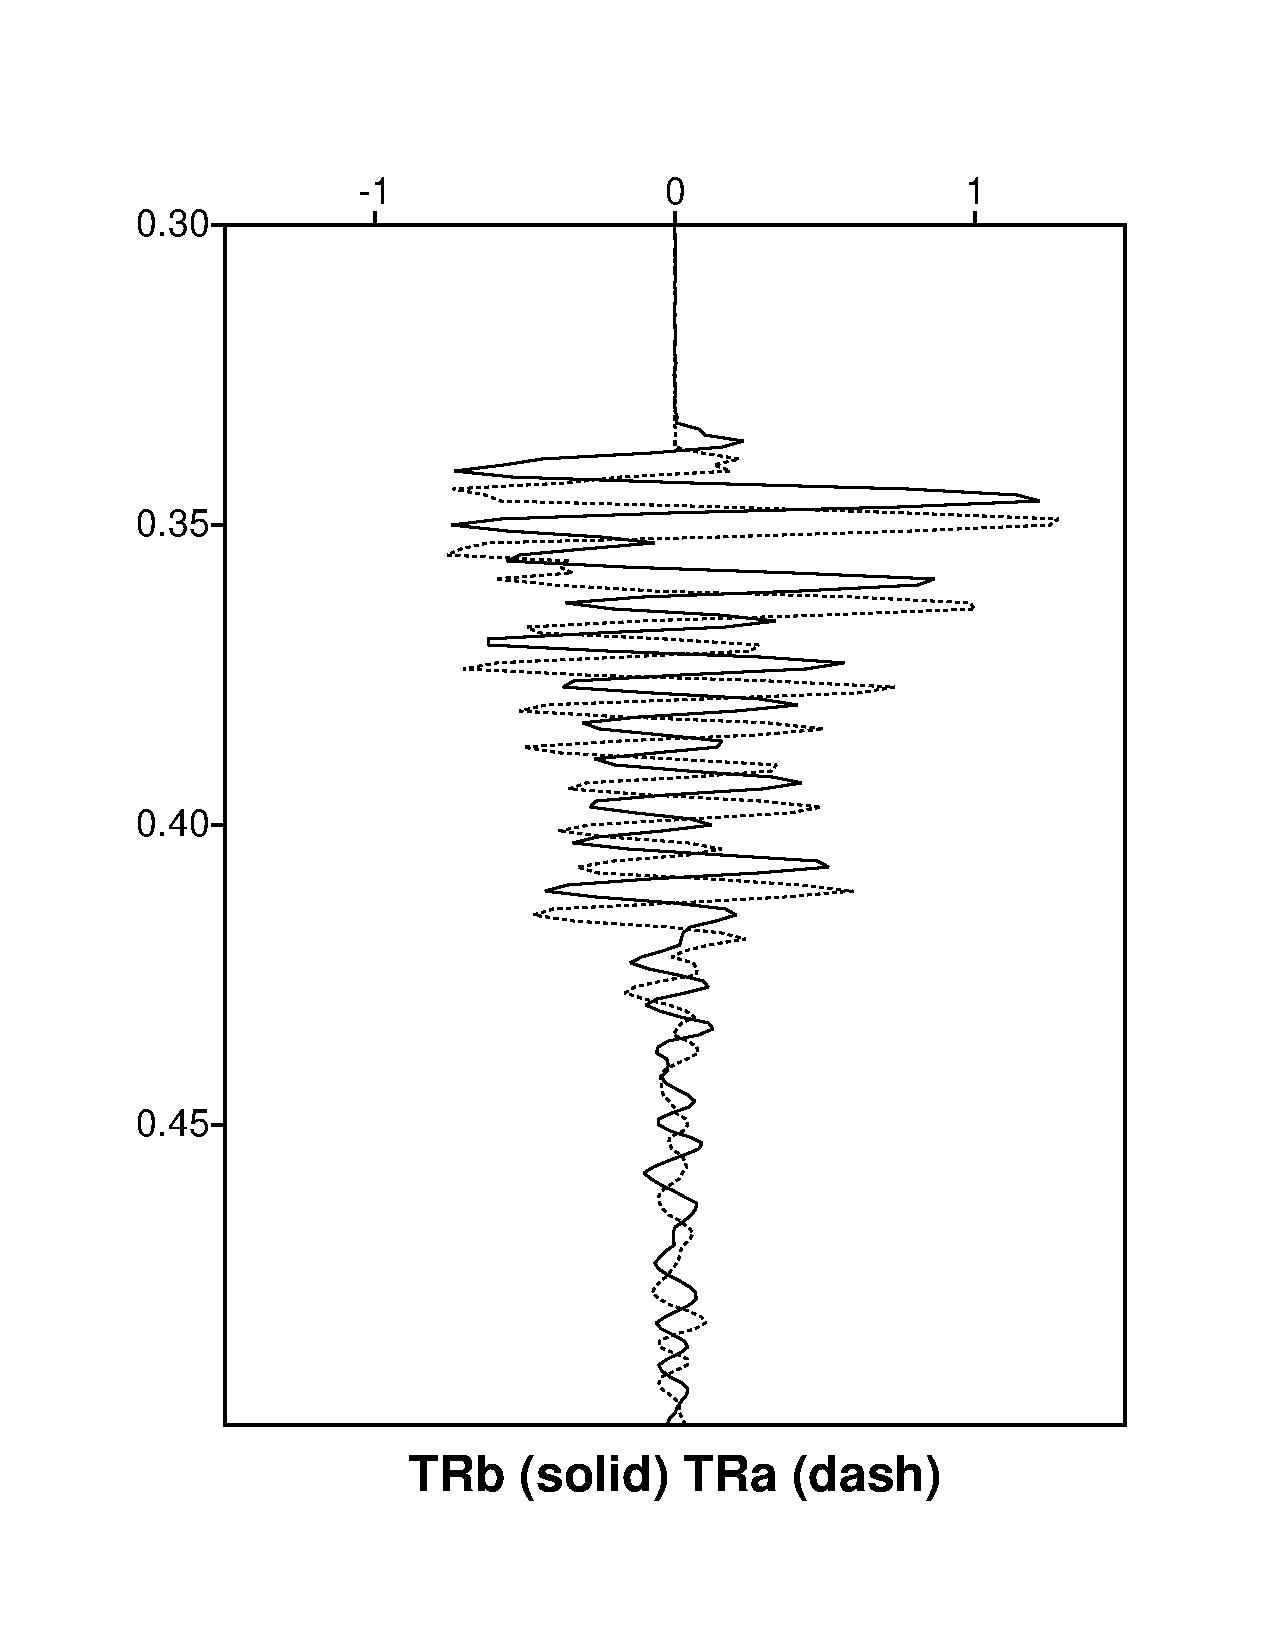
\includegraphics[width=0.45\textwidth]{Fig/fig1}
%    \label{fig:fig1}}\\
%    \subfloat[]{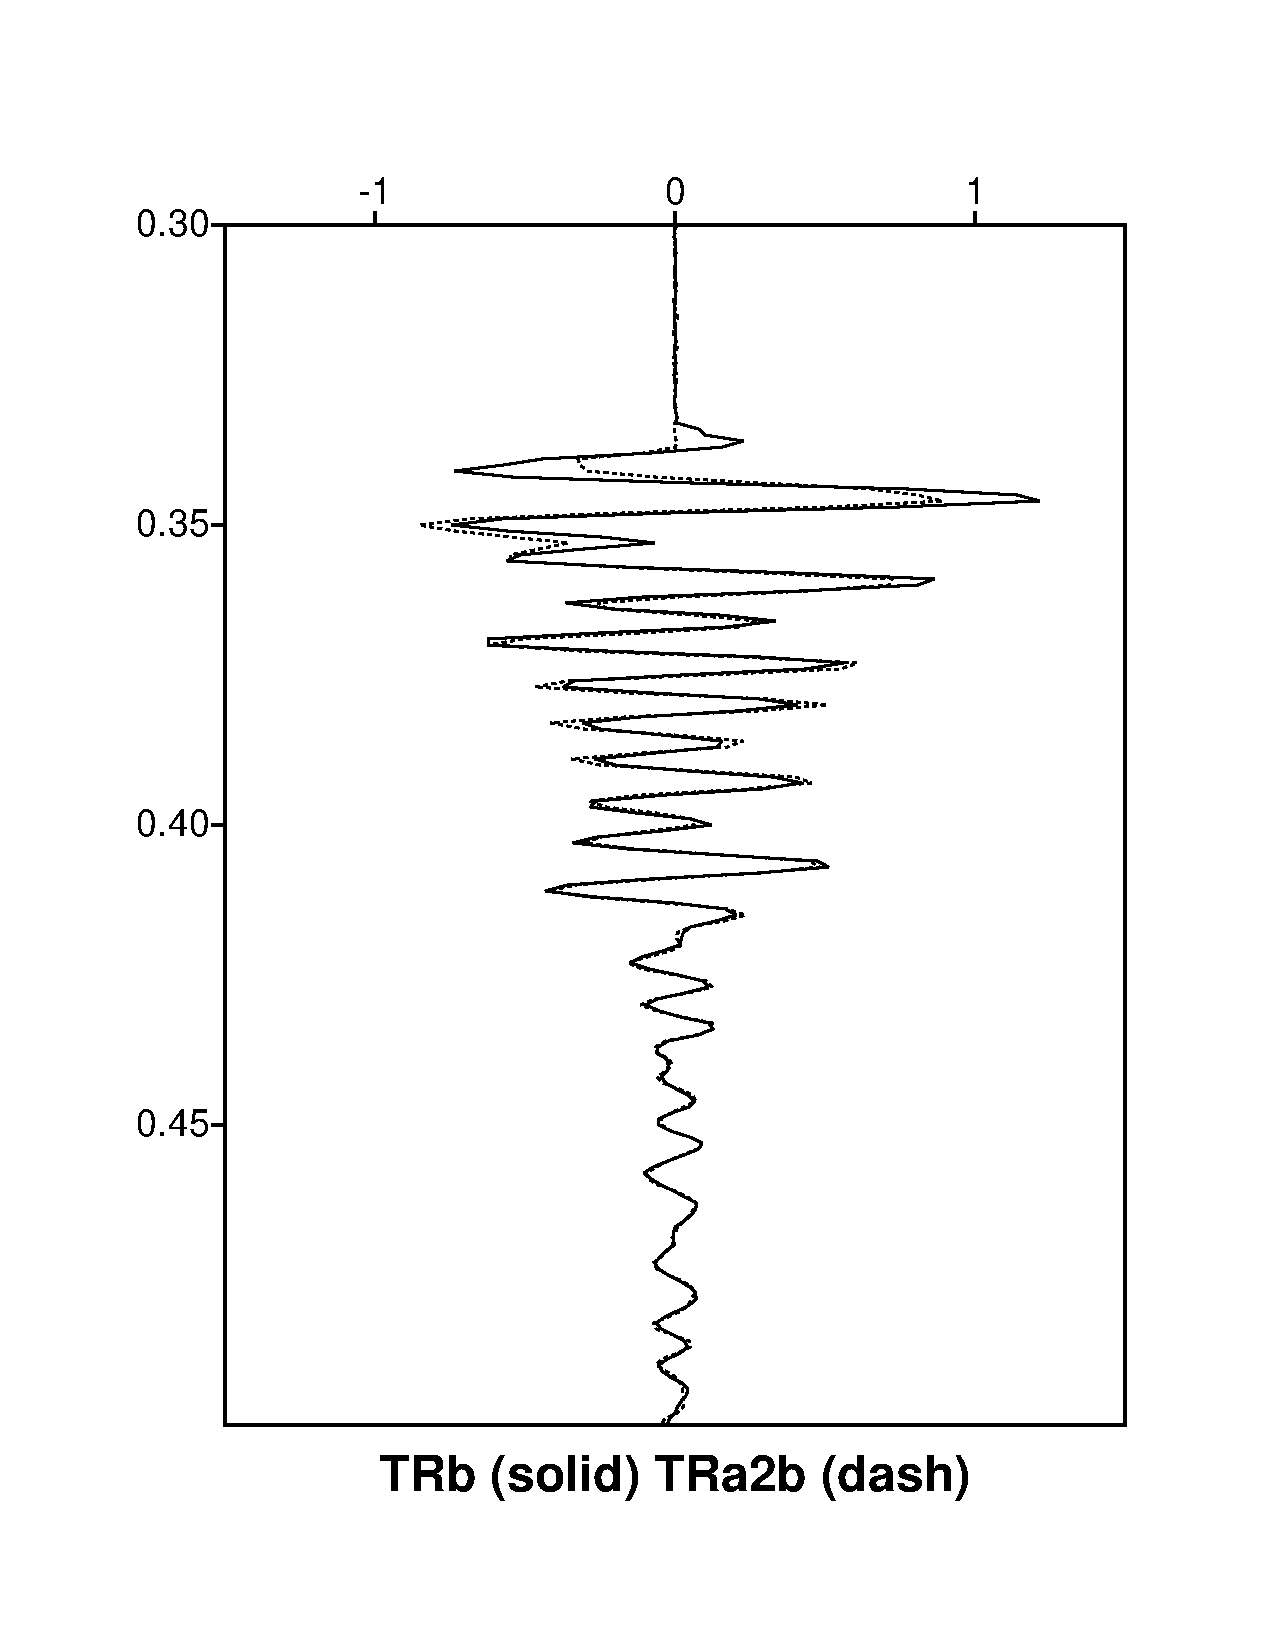
\includegraphics[width=0.45\textwidth]{Fig/fig2}
%    \label{fig:fig2}}\\
%	\caption{(a) Caption a. (b) Caption b.}
%	\label{fig:fig1,fig2}
%\end{figure*}

%\begin{table}[h]
%\caption{Table caption}
%\begin{center}
%     \begin{tabular}{|c|c|c|c|c|c|} 
%	  \hline Column1 (unit)  & Column2 (unit) & Column3 (unit) \\ 
%	  \hline 1 & 2  & 3 \\
%       \hline
%    \end{tabular} 
%\end{center}
%\label{tbl:table1}
%\end{table}

